\section{ОБЗОР ЛИТЕРАТУРЫ}
\label{sec:domain}

\subsection{Брокеры сообщений}

Для передачи данных между компонентами в сложной системе используются так называемые брокеры сообщений (англ. message broker).
Это программа, целью которой является приём, хранение и передача сообщений.
Такой подход позволяет осуществить обработку сообщений в режиме реального времени.
Традиционно брокер состоит из следующих компонентов:
\begin{itemize}
    \item Сообщения - совокупность двоичных или текстовых данных, имеющих что-то общее в контексте программы.
     К этим данным перед отправкой может добавляться дополнительная информация, в зависимости от протокола.
    \item Очереди сообщений - объекты, хранящие сообщения в программе;
\end{itemize}

Существует множество брокеров сообщений. Наиболее известные из них:
\begin{itemize}
    \item ActiveMQ;
    \item IBM MQ;
    \item RabbitMQ;
    \item Redis.
\end{itemize}

Для обеспечения схожей функциональности для кластера используется такая платформа, как Apache Kafka~\cite{kafka_documentation_intro}.
Данная платформа позволяет организовать систему публикации/подписки. 
Структура kafka изображена на рисунке ~\ref{pic:lit_review:kafka_structure}.

\begin{figure}
    \centering
    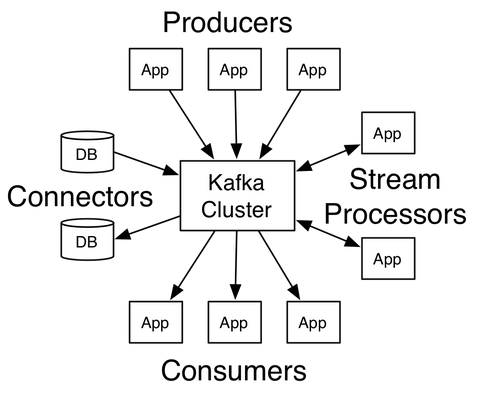
\includegraphics[width=0.7\textwidth]{kafka_structure}
    \caption{Структура брокера сообщений  Apache Kafka~\cite{kafka_documentation_intro}}
    \label{pic:lit_review:kafka_structure}
\end{figure}

Имеется два общих класса приложений, для работы с данной платформой:
\begin{itemize}
    \item приложения, которые осуществляют обмен сообщениями для непосредственно передачи данных между компонентами системы;
    \item приложения, которые преобразуют или реагируют на сообщения.
\end{itemize}

Kafka - это быстрая, расширяемая, долговечная и отказоустойчивая система обмена сообщениями.
Обычно она используется для замены традиционных брокеров сообщений наподобие Java Message Service (JMS) и Advanced Message Queuing Protocol (AMQP) из-за своей высокой пропускной способности, надёжности и использования репликаций.
Может использоваться вместе с такими сервисами, как Storm, Spark, Samza, Flink и другими.
Такая комбинация позволяет анализировать и обрабатывать данные в режиме реального времени.

Рассматриваемая платформа имеет три важных свойства:
\begin{itemize}
    \item публикация и подписка к потоку записей схожа на очередь сообщений;
    \item сохранение потока записей в отказоустойчивой и надёжной системе;
    \item обработка потока записей как только они появляются.
\end{itemize}

А также имеет ещё несколько особенностей, что отличает её от выше упомянутых аналогов:
\begin{itemize}
    \item сбор и мониторинг метрик;
    \item отслеживание активности с помощью веб-сервиса;
    \item использование репликаций в системе логирования.
\end{itemize}

Раздел (англ. partition) в kafke представляет из себя упорядоченную неизменяемую последовательность.
Каждое сообщение в таком разделе ассоциируется с числом, которое обозначает номер сообщения в последовательности раздела.
Это число называется смещением (англ. offset).
Смещение используется для сохранения позиции получателя при получении сообщения.
В свою очередь, каждый топик состоит из одного или более раздела.
Смещение в разделе для каждого получателя хранится в отдельном топике.

Репликации никогда не используются для записи или чтения.
Их единственная задача - заменить лидирующую реплику в случае её отказа.
Один из брокеров в кластере выступает в качестве контроллера, который выбирается автоматически из активных членов кластера.
В задачи этого контроллера входит связывание разделов с брокерами и контроль их отключения.

Разделом всегда владеет один брокер.
Такой брокер называется лидером раздела (англ. leader of the partition).
Остальные брокеры называются последователями (англ. follower).
Все сообщения имеют определённое количество реплик, тем самым при размещении на кластере - такая система становится отказоустойчивой, ведь при выходе из строя некоторой машины - на остальных машинах останутся реплики сообщений, что позволит продолжить работу.
Все последователи постоянно синхронизируются с лидером и копируют актуальную информацию.
Также брокеры делятся на активные и устаревшие.
Устаревшей реплика становится, если в течении определённого времени она не отослала специальный сигнал heartbeat координатору или в течении определённого времени не скопировала актуальную информацию от лидера.
Как только лидер выходит из строя - одна из активных последующих реплик становится новым лидером.

В качестве менеджера выступает zookeeper~\cite{zookeeper_documentation_intro}.
Его структура изображена на рисунке~\ref{pic:lit_review:zookeeper_structure}.                   
С помощью данного сервиса достигается отказоустойчивость системы.

\begin{figure}
    \centering
    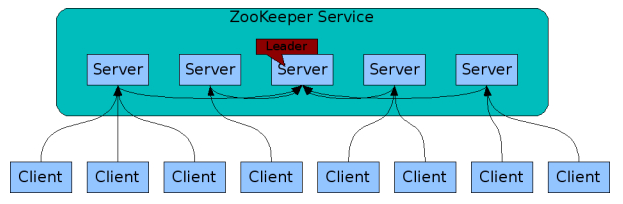
\includegraphics[width=0.7\textwidth]{zookeeper_structure}
    \caption{Структура координирующего сервиса ZooKeeper~\cite{zookeeper_documentation_intro}}
    \label{pic:lit_review:zookeeper_structure}
\end{figure}

\subsection{Контейнеризация}

Для обеспечения работы всех выше перечисленных сервисов, необходим инструмент, который позволит обеспечить работу кластера на одной машине.
Для такой задачи отлично подойдёт Docker~\cite{docker_documentation_intro}.
Docker - это платформа для разработки, развёртки, и запуска приложений в контейнерах.
Использование Linux контейнеров для развёртки приложений называется контейнеризацией.

Контейнеры всё больше и больше становятся популярными по следующим причинам:
\begin{itemize}
    \item гибкость. Даже самые сложные приложения могут быть контейнеризированы;
    \item легковесность. Контейнеры используют и разделяют ядро хоста;
    \item взаимозаменяемость. Возможность развертывать обновления и обновления на лету;
    \item портативность. Возможность собрать локально, разворачивать в облаке, и запускать везде;
    \item расширяемость. Возможность увеличивать и автоматически распределять реплики контейнера;
    \item наращиваемость. Возможность наращивать сервисы на лету.
\end{itemize}

Контейнер запускается с помощью образа.
Образ это исполняемый пакет, который включает в себя всё необходимое для работы приложения - само приложение, окружение, библиотеки, переменные окружения, файлы конфигурациии.
Контейнер это исполняемая сущность образа.

Контейнер изначально работает в Linux и разделяет ядро ​​хост-машины с другими контейнерами.
Он запускает отдельный процесс, занимая не больше памяти, чем любой другой исполняемый файл, что делает его легким.
В отличие от виртуальной машины работает полнофункциональная «гостевая» операционная система с виртуальным доступом к ресурсам хоста через гипервизор.
Как правило, виртуальные машины предоставляют среде больше ресурсов, чем требуется большинству приложений.

Структура работы докера при обычной контейнеризации и с использованием виртуальной машины продемонстрированы на рисунке~\ref{pic:lit_review:docker_vs_vm}

\begin{figure}
    \centering
    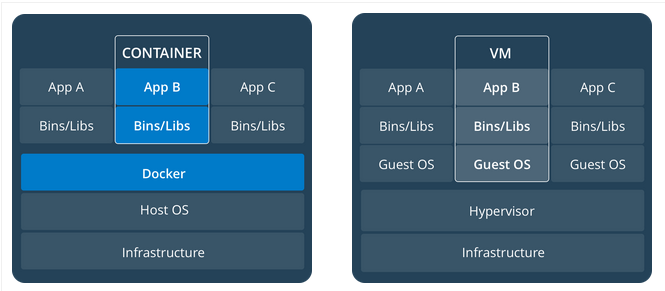
\includegraphics[width=0.7\textwidth]{docker_vs_vm}
    \caption{Работа docker с обычной контейнеризацией и с использованием виртуальной машины~\cite{docker_documentation_intro}}
    \label{pic:lit_review:docker_vs_vm}
\end{figure}

Для обеспечения взаимодействия между контейнерами отлично подходит способ создания виртуальной сети, в которой и запускаются необходимые контейнеры, а также метод пробрасыввания портов, что позволит по необходимому порту пересылать данные между запущенными контейнерами.
Также существует более удобный вариант работы с несколькими контейнерами - docker-compose.
Данный инструмент позволяет удобно оформить настройки планируемого кластера с помощью файла конфигурации.
Благодаря таким инструментам есть возможности добиться работы системы, идентичной в реальных условиях, когда вся эта система будет размещена на полноценном кластере.

\subsection{Произведение вычислений}

Для обработки вычислений на кластере существует отличный продукт под названием Apache Spark~\cite{spark_documentation_intro}.
Apache Spark — это фреймворк с помощью которого можно создавать приложения для обработки данных на кластере.
Он отвечает за распределенное по всему кластеру выполнение приложения.
Данный фреймворк раскидывает код по всем узлам кластера, разбивает на подзадачи, создаёт план их выполнения и следит за их выполнением.
Если на каком либо узле произошел сбой, и подзадача завершилась ошибкой, то она будет перезапущена.
Для данной цели в кластере определяется мастер (англ. spark-master) и рабочие (англ. spark-worker).
Мастер отправляет приложение на рабочие машины и отслеживает их выполнение.
Когда рабочий завершит обработку своей задачи, он отсылает результат обратно на мастер~\cite{spark_architecture_overview}.
Архитектура Apache Spark представлена на рисунке~\ref{pic:lit_review:spark_architecture}.

\begin{figure}
    \centering
    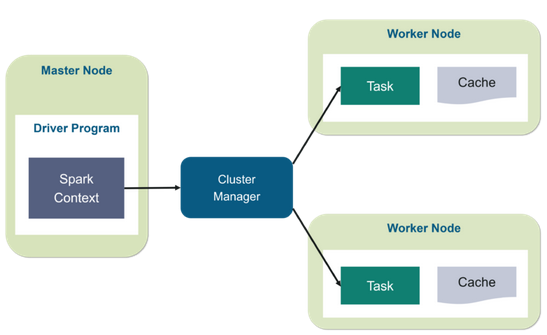
\includegraphics[width=0.7\textwidth]{spark_architecture}
    \caption{Архитектура Apache Spark~\cite{spark_architecture_overview}}
    \label{pic:lit_review:spark_architecture}
\end{figure}

Результаты вычислений представляются в виде RDD (англ. Resilient Distributed Dataset). 
В актуальных версиях spark также применяются аналоги RDD, которые имеют другую структуру и интерфейс (DataFrame и DataSet).
Эти объекты являются ленивыми и вычисляются только на этапе исполнения.
Для отказоустойчивости все вычисления представляют из себя направленный ацикличный граф, благодаря которому, из предыдущих результатов всегда можно получить последующий.
Благодаря такому подходу при потере результатов текущих вычислений есть возможность их восстановить из предыдущих.

Все операции над RDD подразделяются на:
\begin{itemize}
    \item трансформации;
    \item действия.
\end{itemize}

Трансформация - преобразование, результатом которого является новый RDD. 
Примерами такого преобразования служат функции map и filter.
Действия - операции, применяемые для материализации результата.
Например сохранение в файл или подсчёт количества записей.

spark поддерживает несколько менеджеров кластера:
\begin{itemize}
    \item автономный (англ. standalone). Простой кластерный менеджер, включённый в spark, что позволяет легко развернуть кластер;
    \item Apache Mesos. Общий кластерный менеджер, который также может запускать Hadoop MapReduce и сервисные приложения;
    \item Hadoop YARN. Ресурсный менеджер, используемый в Hadoop 2;
    \item Kubernetes. Система с открытым исходным кодом для автоматизации развёртки, расширения, и управления конейнтеризированными приложениями.
\end{itemize}

При использовании автономного режима - spark самостоятельно будет контролировать ресурсы кластера и запускать приложения.
Локальный режим запускает приложение как один процесс, что позволяет осуществлять отладку.
Yarn это ресурсный менеджер, входящий в экосистему Hadoop~\cite{hadoop_difinitive_guide}.
Mesos это альтернативный менеджер ресурсов кластера.

При работе в автономном режиме, в качестве рабочих узлов используются ядра машины, на которой запускается приложение.
Количество используемых ядер можно ограничить.
    
\subsection{Визуализация данных}

Для визуализации данных существует такой проект, как Apache Zeppelin~\cite{zeppelin_documentation_intro}.
Apache Zeppelin - это веб-приложение наподобие проекта Jupyter Notebook с открытым исходным кодом, который  позволяет осуществлять интерактивный анализ данных.
Данный notebook интегрирован с такими распределёнными, универсальными системами, как Apache Spark, Apache Flink и с многими другими.
Zeppelin позволяет создавать удобные, интерактивные документы с помощью таких языков, как SQL, Scala, R и Python, напрямую из браузера.

Особенности данного проекта:
\begin{itemize}
    \item интерактивный интерфейс. Apache Zeppelin имеет интерактивный интерфейс, который позволяет мгновенно увидеть результаты анализа;
    \item использование браузера. Создание интерактивных документов напрямую в браузере, что позволяет использовать его удалённо. Также это позволяет эксперементировать с различными типами диаграмм для представления результатов;
	\item интегрирование. Интеграция со многими различными инструментами с открытым исходным кодом, предназначенными для обработки большого количества данных. Например Spark, Flink, Hive, Ignite, Lens и Tajo;
	\item динамические формы. Динамическое создание форм ввода прямо в интерактивном документе;
    \item сотрудничество и обмен. Сообщество разработчиков предоставляет доступ к новым источникам данных, которые постоянно добавляются и распространяются через их лицензию Apache 2.0 с открытым исходным кодом;
    \item интерпретатор. Концепция интерпретатора позволяет использовать любой язык либо приложения для обработки данных. В настоящее время Apache Zeppelin поддерживает множество интерпретаторов, таких как: Apache Spark, Python, JDBC, Markdown и Shell.
\end{itemize}

Благодаря таким свойствам, данный инструмент отлично подойдёт для интерактивного способа представления данных.

Apache Zeppelin в своём составе имеет интерпретатор Spark, что позволяет сразу в интерактивном документе запускать Spark приложения.
Также благодаря самому Zeppelin есть возможность сериализировать и передавать данные между разными интерпретаторами, что позволяет использовать несколько интерпретаторов при обрабатывке данных.
В интерактивном документе можно использовать встроенные средства для визуализации данных, что позволяет сразу в удобной форме увидеть преобразованные данные.


\subsection{Непрерывная интеграция}

Так как разрабатываемый продукт является проектом с открытым исходным кодом, то важной частью процесса разработки является процесс непрерывной интеграции.
Для данной цели используется такой инструмент, как Jenkins~\cite{jenkins_documentation}.
Данный инструмент из себя представляет Java веб-приложение, которое позволяет запускать заготовленные команды, и отслеживать их исполнение.
С помощью Jenkins появляется возможность проводить интеграционные тесты для какой-либо ветки в системе Git из удалённого репозитория.

Команды, которые должен исполнить Jenkins прописываются либо прямо в настройках, либо берутся из удалённого репозитория, к которому Jenkins имеет доступ.
Все команды исполняются на машине, в которой запущена данная платформа.
Однако для создания определённого системного окружения отлично подойдёт Docker и его аналог docker-compose, которые были рассмотрены выше.

С помощью такой системы непрерывной интеграции, всегда можно узнать работоспособность конкретной версии продукта.
Эта возможность крайне важна при разработке сообществом.

В качестве альтернативы Jenkins можно использовать GitLab.
Рассматриваемый сервис имеет инструменты для конфигурирования и использования непрерывной интеграции.